\chapter{Thiết kế kiến trúc hệ thống}
\section{Kiến trúc Sạch (Clean Architecture)}
Dự án được thiết kế theo mô hình kiến trúc sạch (Clean Architecture) được xây dựng dựa trên tư tưởng "độc lập" và kết hợp với các nguyên lý thiết kế hướng đối tượng (Dependency Inversion) \\

\begin{figure}[h]
    \centering
    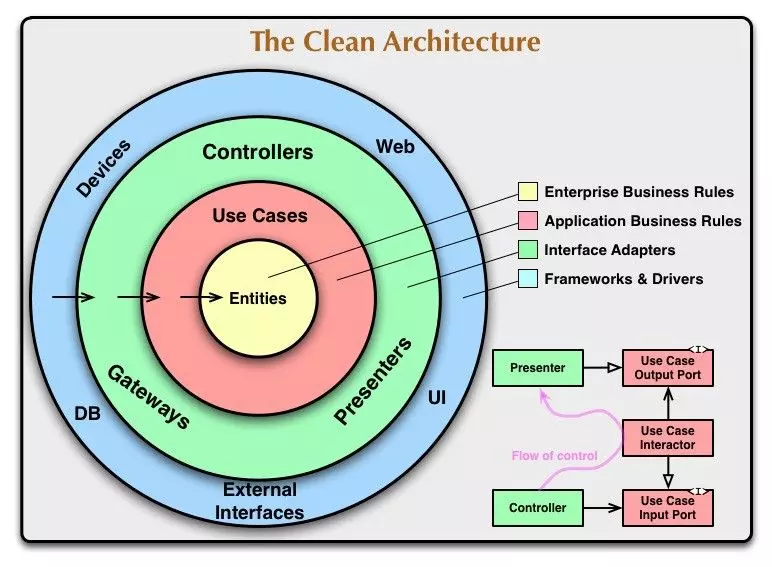
\includegraphics[scale = 0.5]{img/design/clean2.png}
    \vspace{1cm}
    \caption{Clean Architecture}
    \label{fig:taskAssignment}
\end{figure}
\noindent
Kiến trúc của Clean Architecture được chia thành 4 layer với một quy tắc phụ thuộc, các layer ở bên trong không cần biết về bất kì điều gì về các layer bên ngoài:
\begin{itemize}
    \item Entities: là khái niệm dùng để mô tả các Business Logic. Đây là layer quan trọng nhất, là nơi thực hiện giải quyết các vấn đề - mục đích khi xây dựng app. Layer này không chứa bất kỳ một framework nào, bạn có thể chạy nó mà không cần emulator. Nó giúp dễ dàng kiểm tra, bảo trì và phát triển phần bussiness logic.
    \item Use case : chứa các rule liên quan trực tiếp tới ứng dụng cục bộ (application-specific business rules).
    \item Interface Adapter : tập hợp các adapter phục vụ quá trình tương tác với các công nghệ.
    \item Framework and Drivers : chứa các công cụ về cơ sở dữ liệu và các framework, thông thường bạn sẽ không phải lập trình nhiều ở tầng này. Tuy nhiên cần chắc chắn về mức ưu tiên sử dụng các công cụ này trong project.
\end{itemize}
\begin{figure}[h]
    \centering
    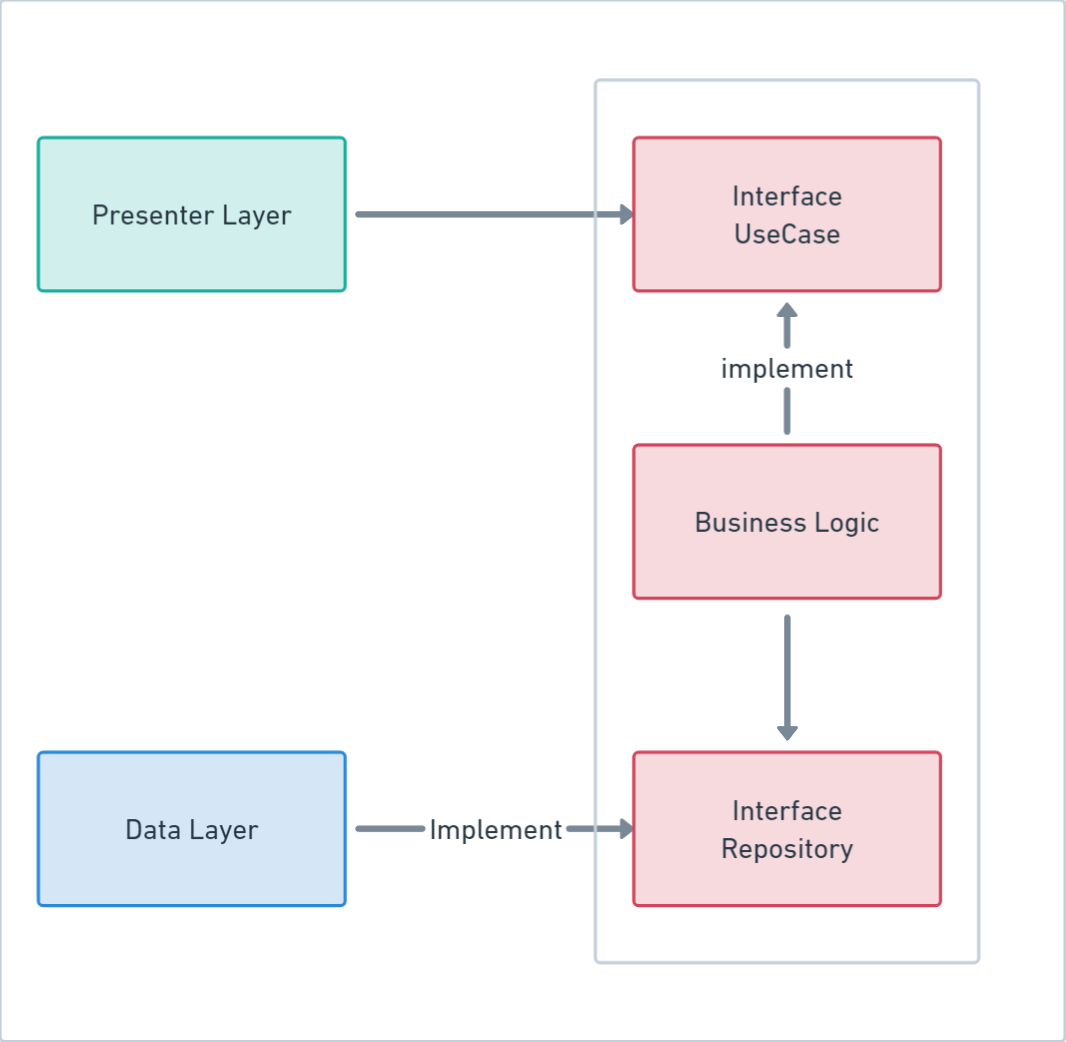
\includegraphics[scale = 0.3]{img/design/clean.png}
    \vspace{1cm}
    \caption{Clean Architecture với mô hình phân lớp áp dụng Dependency Inversion}
    \label{fig:taskAssignment}
\end{figure}
\noindent
Trong dự án này, Ta sẽ chia hệ thống thành 3 lớp chính, áp dựng nguyên tắc Dependency Inversion của Clean Architecture 
\begin{itemize}
    \item Presenter Layer: Đây là tầng nhận các yêu cầu và trả phản hồi cho người dùng, chúng tương tác với tầng nghiệp vụ (Business Layer) thông qua một UseCase Interface.
    \item Business Logic: Đây là tầng thiện thực Usecase Interface, thực hiện các nghiệp vụ, logic chính của hệ thống. Ở tầng này, việc truy vấn vào cơ sở dữ liệu được gọi thông qua một Interface Repository.
    \item Data Layer: Đây là tầng cuối cùng của hệ thống, hiện thực các chức năng truy vấn vào cơ sở dữ liệu dựa theo thuộc tính của mỗi thực thể, chúng được hiện thực dựa trên interface Repository
\end{itemize}
Như đã trình bày ở trên, trong kiến trúc này, các tầng không tham chiếu trực tiếp với nhau mà qua một giao diện (interface) của mỗi lớp. Mỗi lớp của một tầng bên trong không trực tiếp tham chiếu đến class bên ngoài.
\newpage
\section{Thiết kế hệ thống}
\begin{figure}[h]
    \centering
    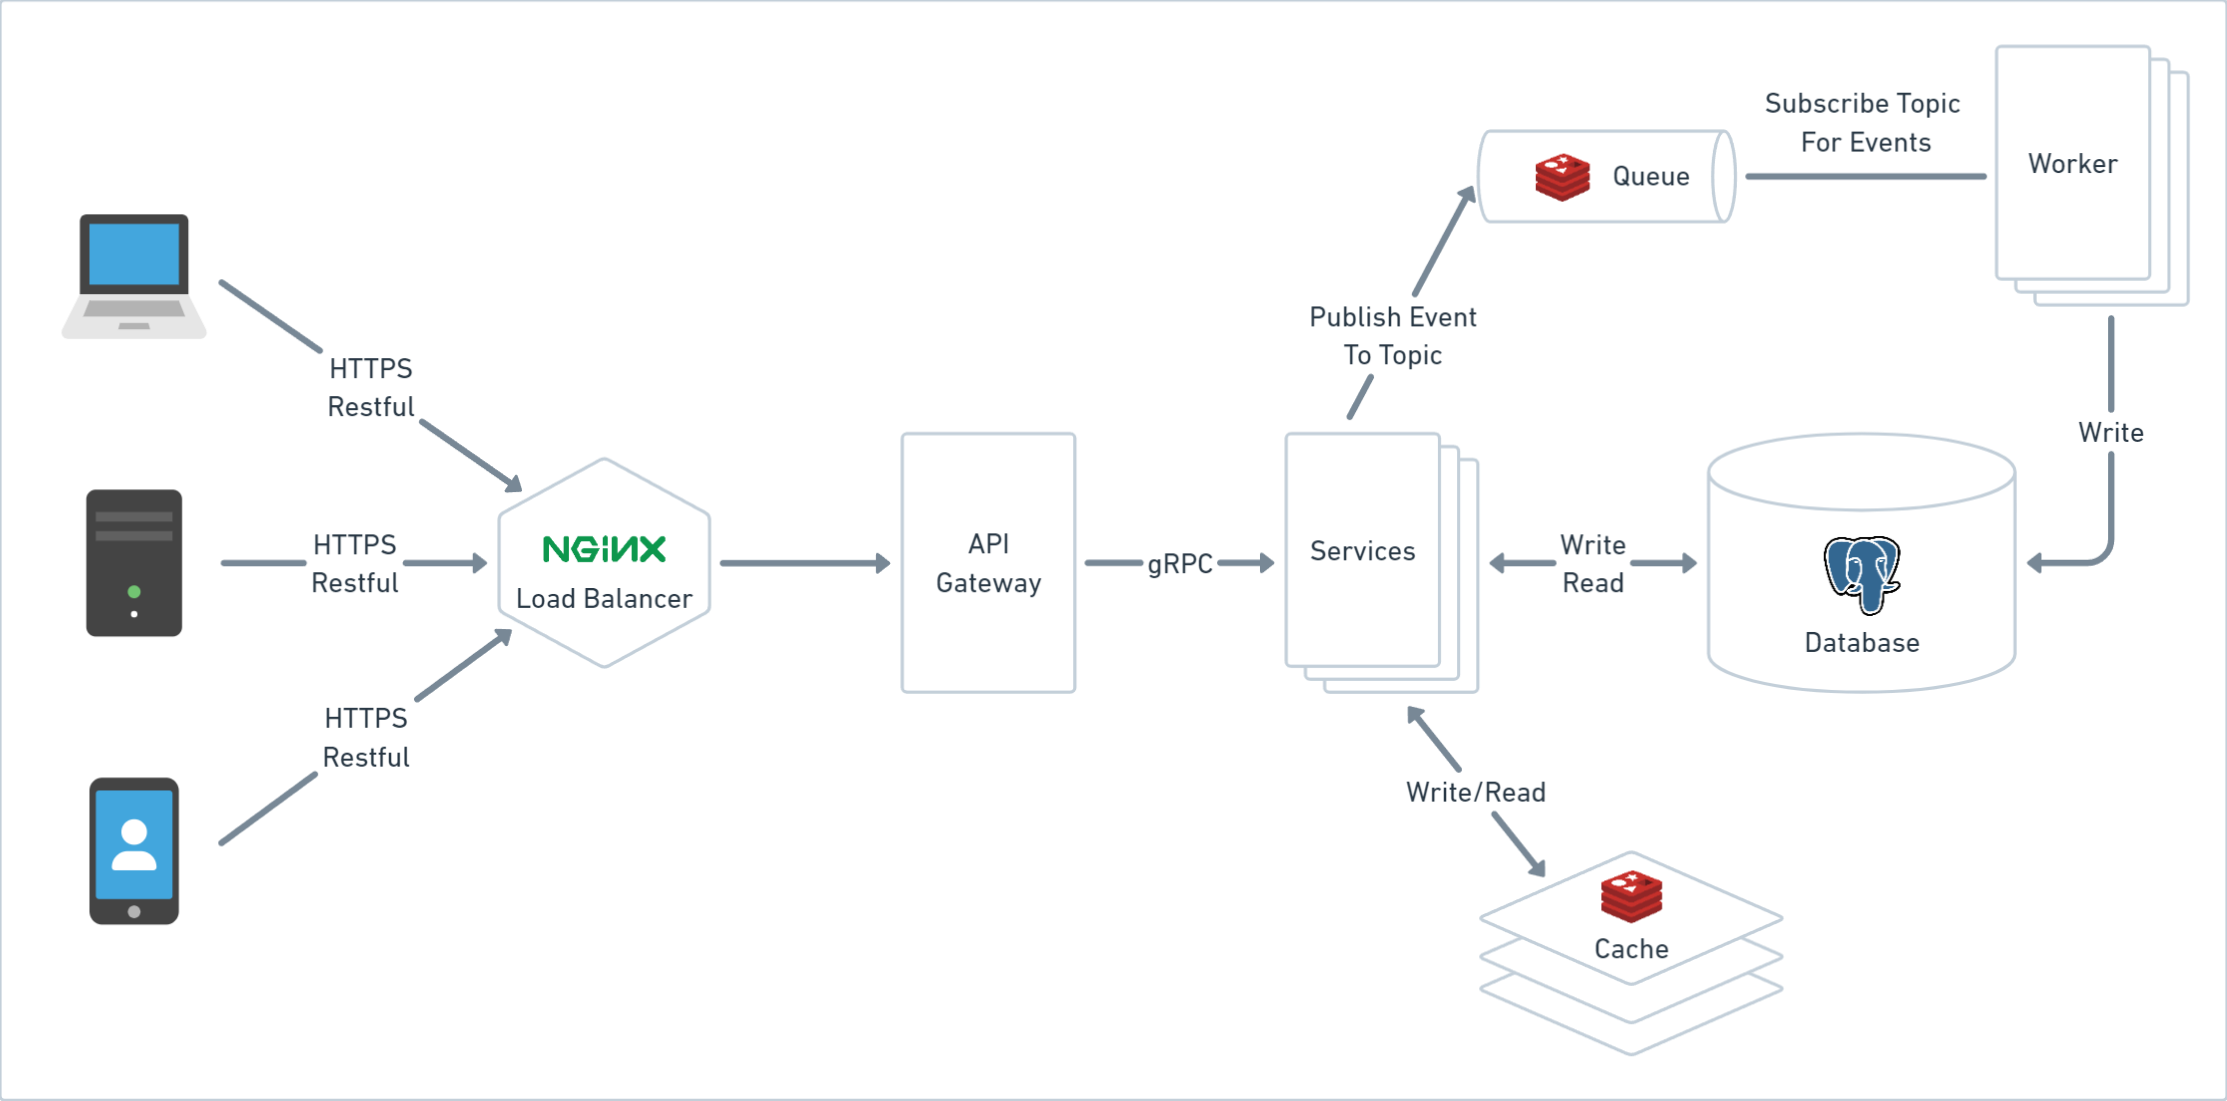
\includegraphics[scale = 0.21]{img/design/system.png}
    \vspace{1cm}
    \caption{System Design cho hoạt động phía máy chủ}
    \label{fig:taskAssignment}
\end{figure}
\noindent
Hệ thống này được thiết kế để đáp ứng một loạt các yêu cầu phức tạp, đồng thời đảm bảo tính linh hoạt và hiệu suất cao. Với kiến trúc phân tán, hệ thống này cho phép tối ưu hóa tài nguyên và mở rộng dễ dàng theo nhu cầu.\\
\\
Các thành phần chính của hệ thống bao gồm các microservices độc lập, chịu trách nhiệm cho các chức năng cụ thể. Các microservices này liên thông thông qua các giao thức tiêu chuẩn, tạo nên một môi trường đồng bộ và ổn định. Hệ thống hỗ trợ việc quản lý lỗi và khôi phục tự động để đảm bảo khả năng hoạt động liên tục.\\
\\
Web server \textbf{NGINX} đóng vai trò như một \textit{reverse proxy server} giúp cho máy chủ phản hồi và phân phát tài nguyên cho các dịch vụ, giúp cho hệ thống ổn định mà không bị quá tải khi có lượng lớn yêu cầu truy cập.\\
\\
Redis đóng vai trò quan trọng trong dự án, vừa là nơi lưu trữ các tác vụ phân tán, vừa đóng vai trò là một bộ nhớ cache, giúp cho việc truy vấn vào cơ sở dữ liệu một cách tối ưu về hiệu suất, hiệu năng.\\
\\
Với khả năng mở rộng linh hoạt, hệ thống này có thể thích ứng với sự thay đổi trong quy mô và yêu cầu, cung cấp một nền tảng mạnh mẽ cho các ứng dụng và dịch vụ đa dạng.
\newpage
\section{Cơ sở dữ liệu}
\begin{figure}[h]
    \centering
    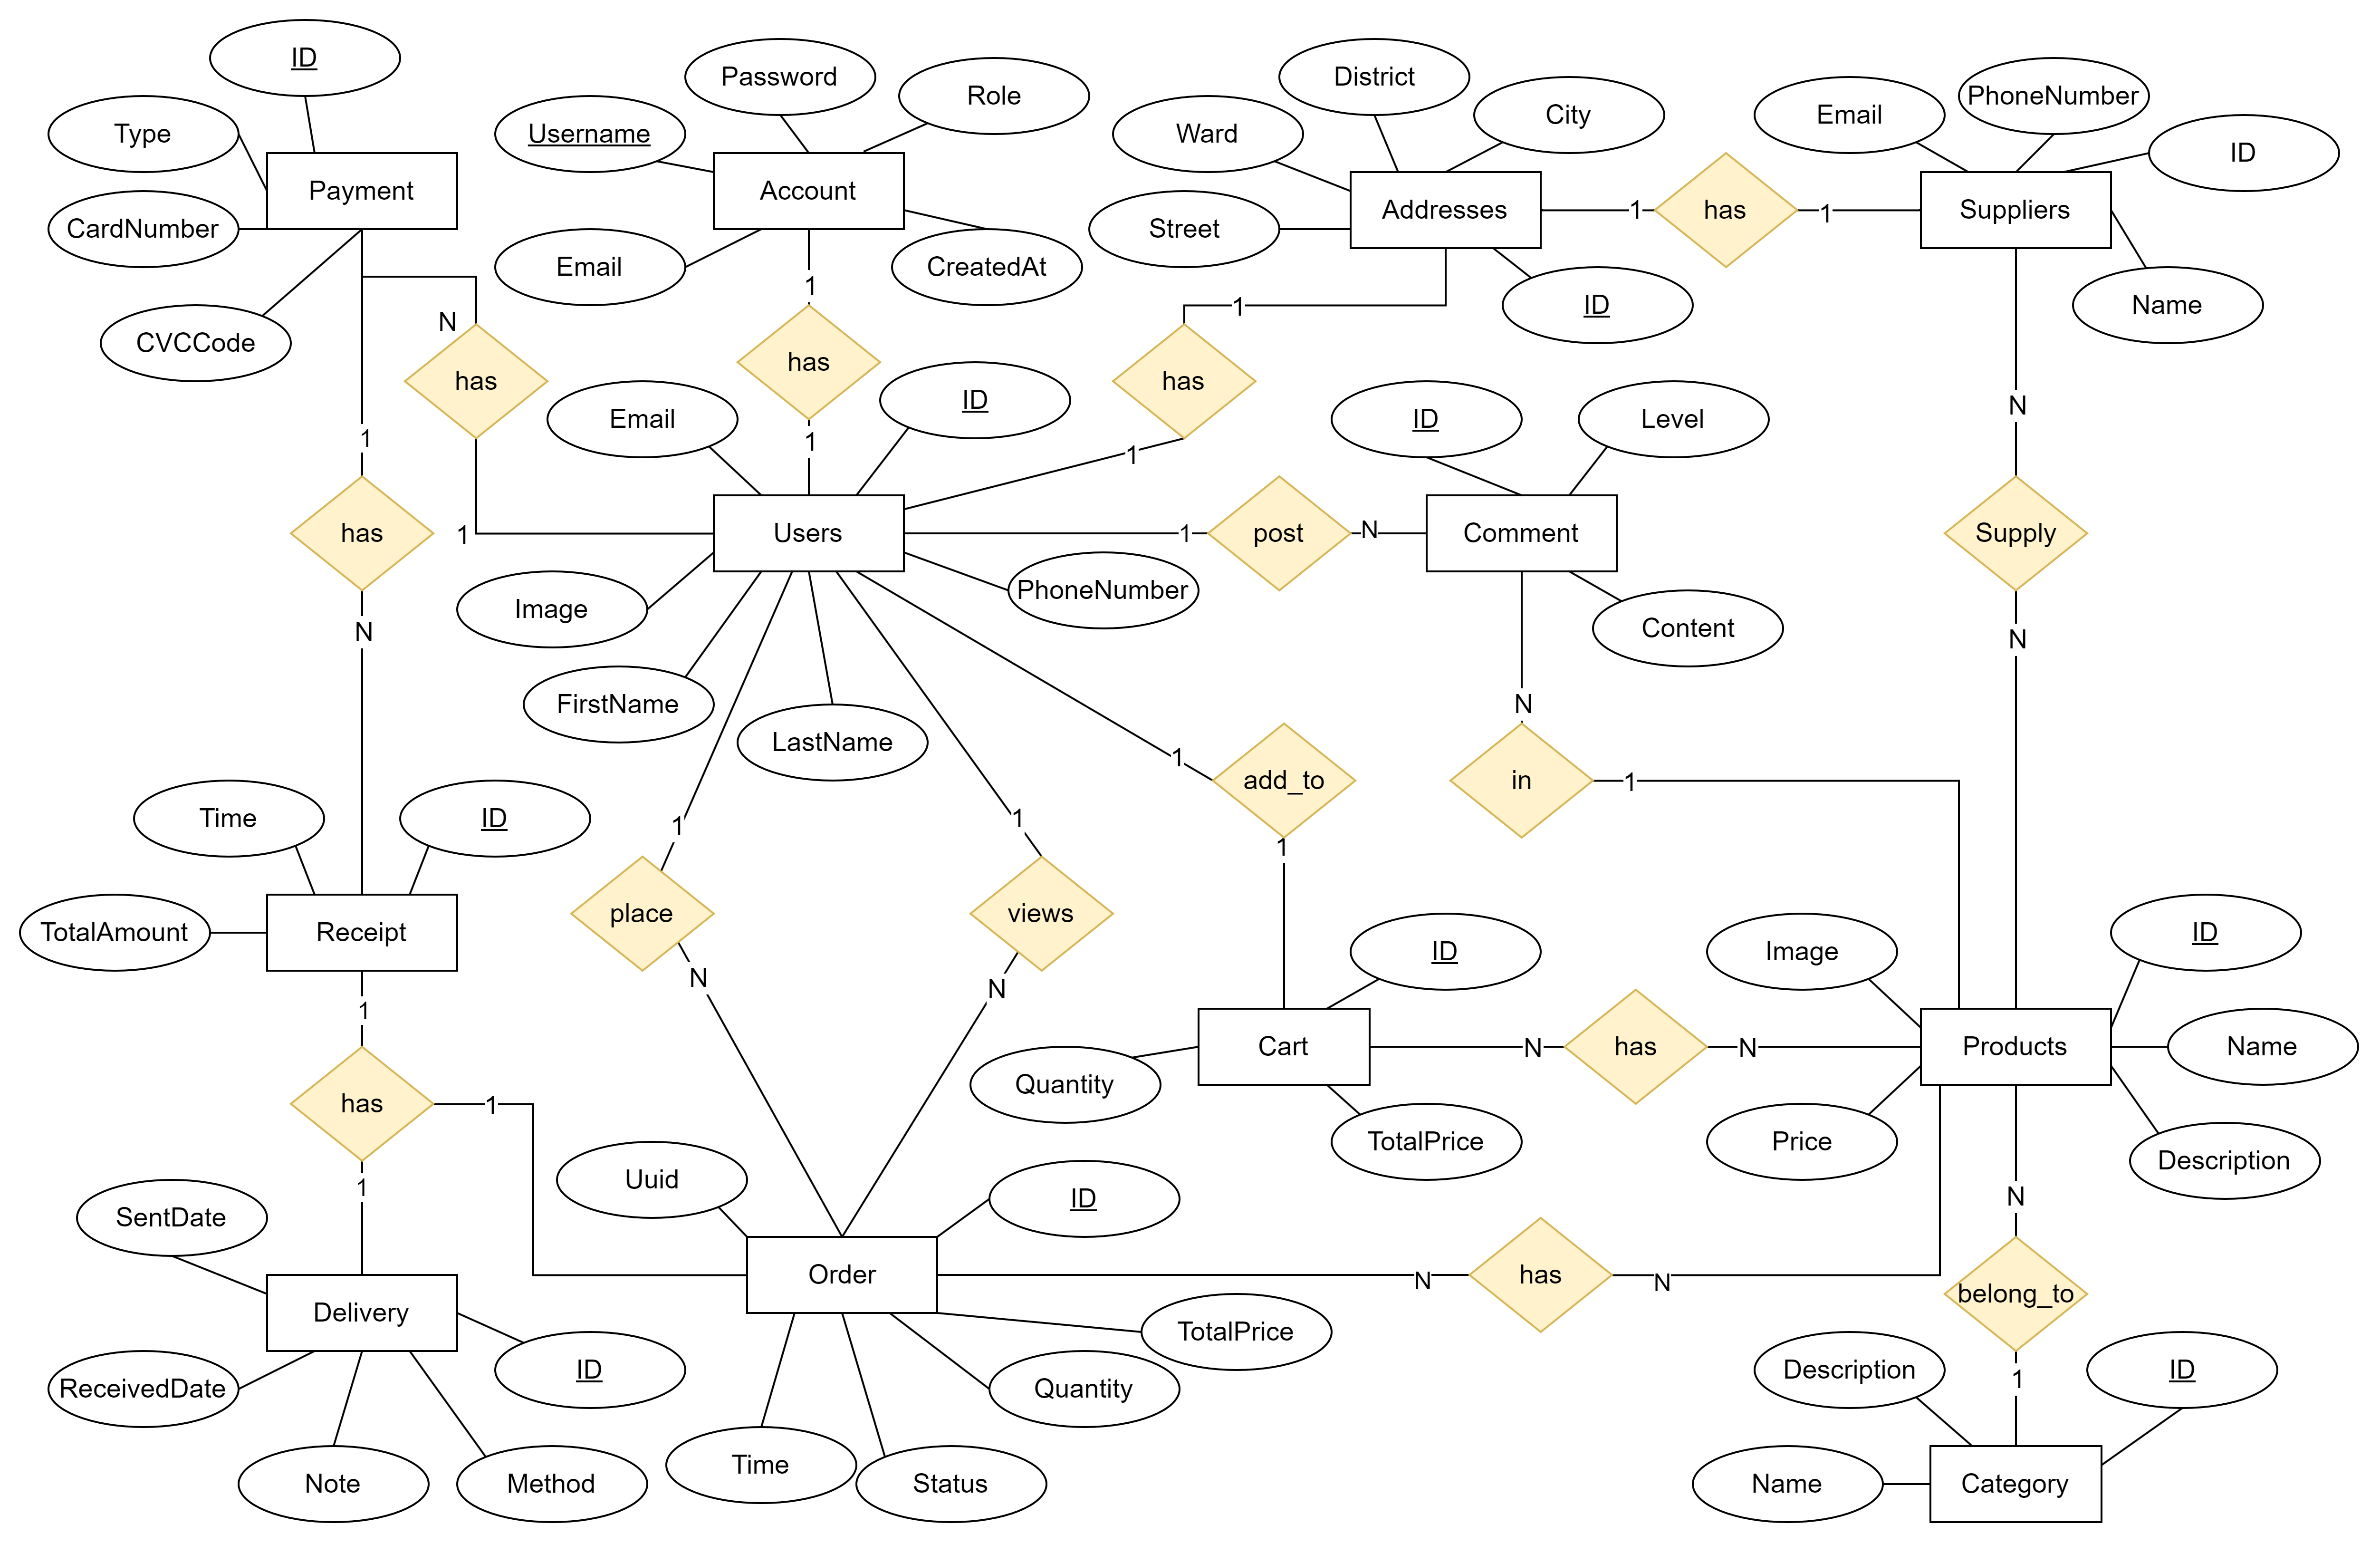
\includegraphics[scale = 0.10]{img/erd.png}
    \vspace{1cm}
    \caption{Lược đồ thực thể - mối quan hệ trong Database}
    \label{fig:taskAssignment}
\end{figure}
\subsection{Các ràng buộc chính về các thực thể trong dự án}
\begin{itemize}
    \item \textbf{Users - has - Addresses}:  Một người dùng \textbf{(Users)} có một địa chỉ \textbf{(Addresses)} và ngược lại, Một địa chỉ chỉ được tạo ra bởi một người dùng.
    
    \item \textbf{Users - has - Account}: Một người dùng chỉ có một tài khoản \textbf{(Accounts)} duy nhất, và ngược lại, một tài khoản chỉ có thể được tạo ra bởi một người dùng 
    
    \item \textbf{Users - has - Payment}: Một người dùng \textbf{(Users)} cũng có thể có nhiều phương thức thanh toán \textbf{(Payment)}, nhưng một phương thức thanh toán chỉ có thể được thêm vào bởi một người dùng duy nhẩt.
    
    \item \textbf{Payment - has - Receipt}: Một phương thức thanh toán \textbf{(Payment)} có thể thanh toán cho nhiều hóa đơn \textbf{(Receipt)} nhưng một hóa đơn chỉ có thể thanh toán bởi một phương thức thanh toán nhất định.
    
    \item \textbf{Users - place - Order}: Người dùng \textbf{(Users)} có thể đặt nhiều đơn hàng \textbf{(Order)}, nhưng đơn hàng chỉ được đặt bởi một người dùng duy nhất.
    
    \item \textbf{Users - views - Order}: cũng có thể xem nhiều đơn hàng\textbf{(Order)}, và Đơn hàng chỉ xem được bởi một người dùng duy nhất.
    
    \item \textbf{Users - post - Comment}: Người dùng cũng có thể đăng nhiều bình luận \textbf{(Comment)}, và mỗi Bình luận chỉ được đăng bởi một người.

    \item \textbf{Users - add\_to - Cart}:  Một người dùng \textbf{(Users)} chỉ có một giỏ hàng duy nhất, và ngược lại.
    
    \item \textbf{Receipt - has - Delivery}: Một Hóa đơn \textbf{(Receipt)} chỉ có một Phương thức vận chuyển \textbf{(Delevery)} duy nhất, và ngược lại

    \item \textbf{Receipt - has - Order}: Một hóa đơn \textbf{(Receipt)} thì chỉ có một đơn hàng \textbf{(Order)} duy nhất, và ngược lại

    \item \textbf{Order - has - Delivery}: Một đơn hàng \textbf{(Order)} chỉ có một phương thức vận chuyển \textbf{(Delivery)} duy nhất, và ngược lại 

    \item \textbf{Order - Has - Product}: Một đơn hàng \textbf{(Order)} có thể có nhiều sản phẩm \textbf{Product} trong đơn hàng và ngược lại, sản phẩm cũng có thể nằm trong nhiều đơn hàng khác nhau.

    \item \textbf{Cart - has - Products}: Một giỏ hàng có thể có nhiều sản phẩm trong giỏ. Và ngược lại, Sản phẩm cũng có thể nằm trong nhiều giỏ hàng.

    \item \textbf{Comment - in - Products}: Một bình luận \textbf{(Comment)} chỉ nằm trong một sản phẩm nhất định, nhưng một sản phẩm có thể có nhiều bình luận được người dùng đăng tải.

    \item \textbf{Supplier - has - Addresses}: Nhà cung cấp \textbf{(Supplier)} chỉ có một địa chỉ được lưu trên hệ thống, và ngược lại, một địa chỉ là địa chỉ của một trong hai thực thể, Người dùng và nhà cung cấp.

    \item \textbf{Supplier - supply - Products}: Nhà cung cấp có thể cung cấp nhiều sản phẩm. và sản phẩm cũng được cung cấp bởi nhiều nhà cung cấp.

    \item \textbf{Category - belong\_to - Products}: Một sản phẩm được phân loại thành một Danh mục nhất định, nhưng một Danh mục có thể nằm trong nhiều sản phẩm
\end{itemize} 

\newpage
\subsection{Các thực thể chính}
\begin{figure}[h]
    \centering
    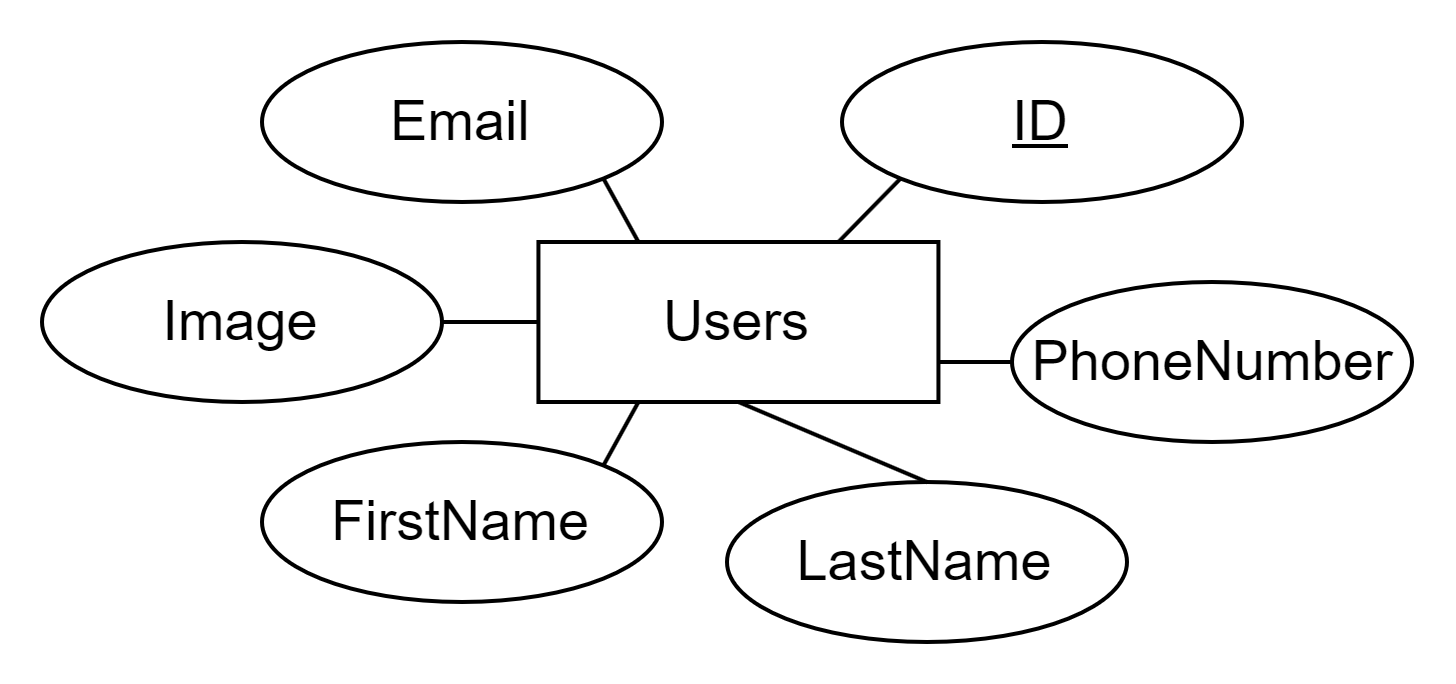
\includegraphics[scale = 0.20]{img/db/users.png}
    \vspace{1cm}
    \caption{Chi tiết thực thể \textbf{Users}}
    \label{fig:taskAssignment}
\end{figure}
Các thuộc tính chính của thực thể \textbf{Users}
\begin{itemize}
    \item Email: Email của người dùng
    \item ID: ID của người dùng, do hệ thống tạo để định danh người dùng
    \item FirstName: Tên của người dùng cung cấp
    \item LastName: Họ của người dùng cung cấp
    \item PhoneNumber: Số điện thoại mà người dùng cung cấp
    \item Image: Đường dẫn tới hình ảnh đại diện của người dùng
\end{itemize}

\begin{figure}[h]
    \centering
    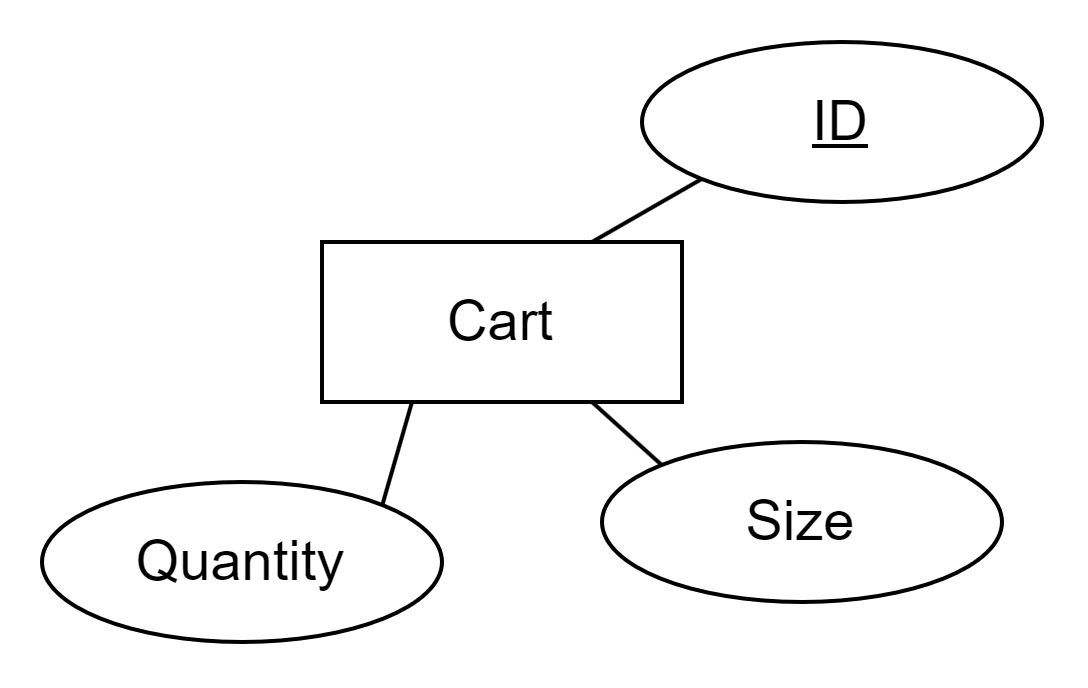
\includegraphics[scale = 0.20]{img/db/cart.png}
    \vspace{1cm}
    \caption{Chi tiết thực thể \textbf{Cart}}
    \label{fig:taskAssignment}
\end{figure}
Các thuộc tính chính của thực thể \textbf{Cart}
\begin{itemize}
    \item Quantity: Tổng số tiền của giỏ hàng
    \item ID: ID dùng để định danh giỏ hàng
    \item Size: Số lượng hàng trong giỏ
\end{itemize}


\begin{figure}[h]
    \centering
    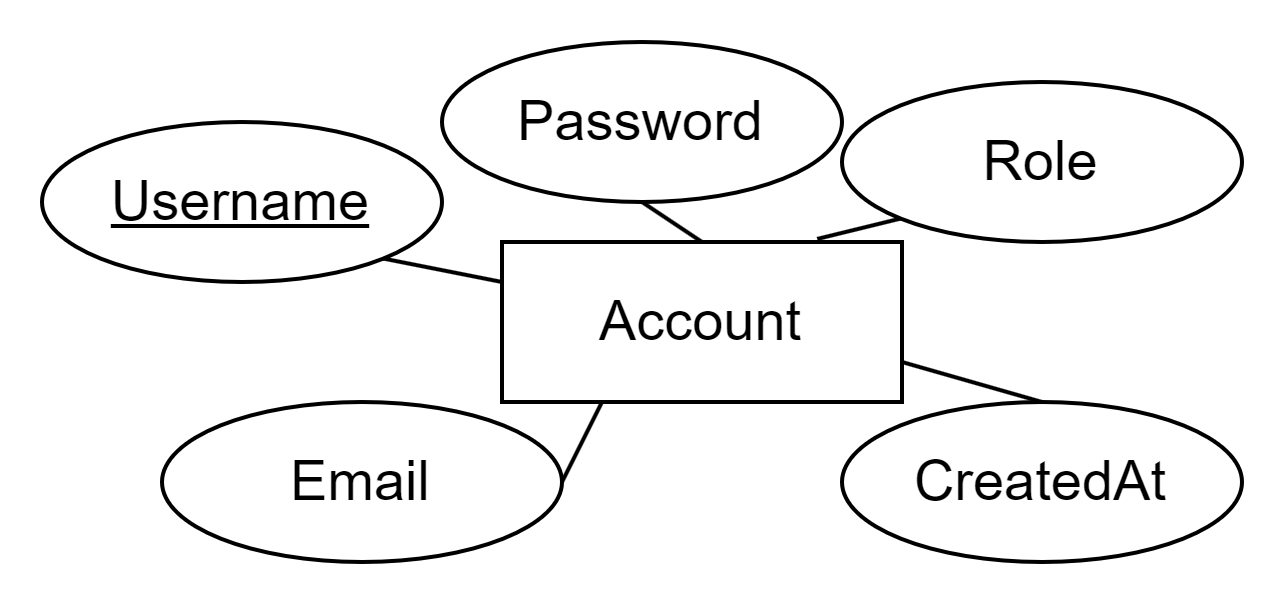
\includegraphics[scale = 0.20]{img/db/account.png}
    \vspace{1cm}
    \caption{Chi tiết thực thể \textbf{Account}}
    \label{fig:taskAssignment}
\end{figure}
Các thuộc tính chính của thực thể \textbf{Account}
\begin{itemize}
    \item Username: Tên đăng nhập của người dùng
    \item Password: Mật khẩu truy cập của người dùng sau khi được mã hóa
    \item Role: Vai trò của người dùng, mặc định là "Customer"
    \item Email: Email của người dùng sử dụng đăng kí tài khoản
    \item CreatedAt: Thời gian người dùng tạo tài khoản 
\end{itemize}

\begin{figure}[h]
    \centering
    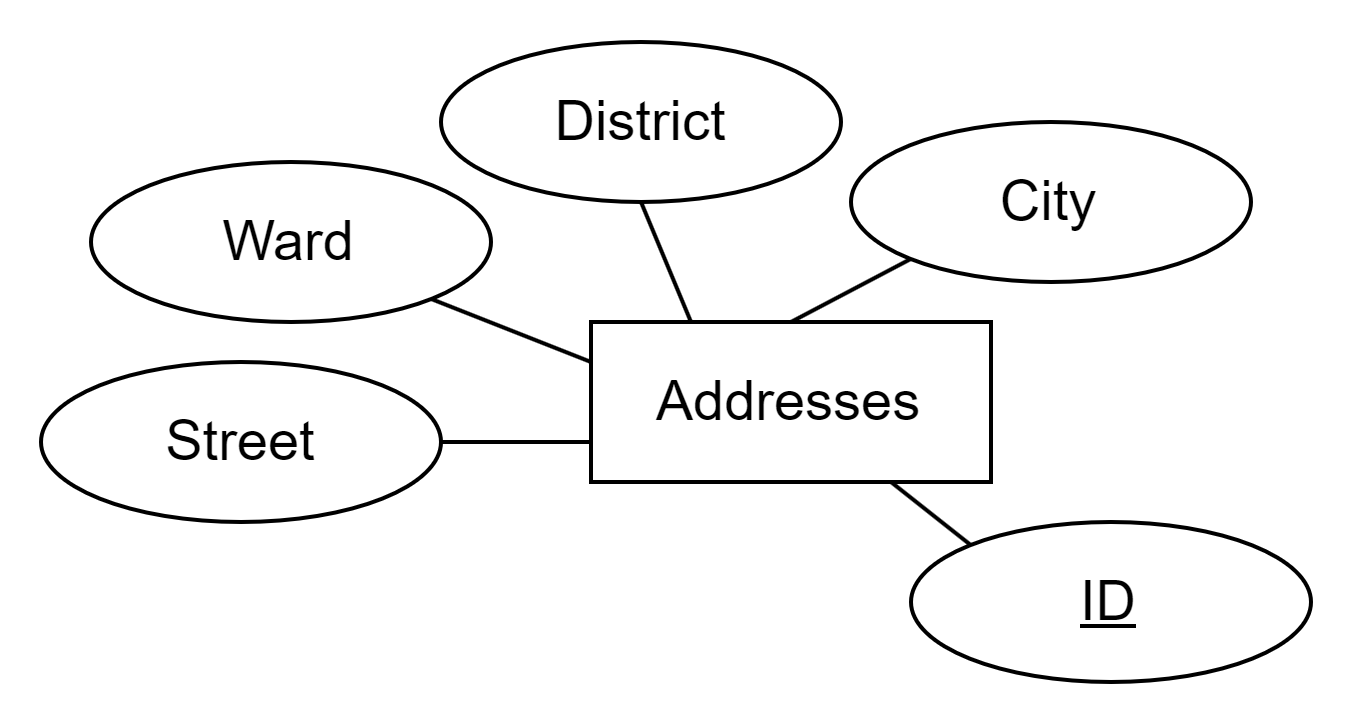
\includegraphics[scale = 0.20]{img/db/addresses.png}
    \vspace{1cm}
    \caption{Chi tiết thực thể \textbf{Addresses}}
    \label{fig:taskAssignment}
\end{figure}
Các thuộc tính chính của thực thể \textbf{Addresses}
\begin{itemize}
    \item District: Quận, huyện
    \item ID: ID định danh địa chỉ
    \item Ward: Phường, xã
    \item Street: Đường
    \item City: Tỉnh, thành phố
\end{itemize}

\begin{figure}[h]
    \centering
    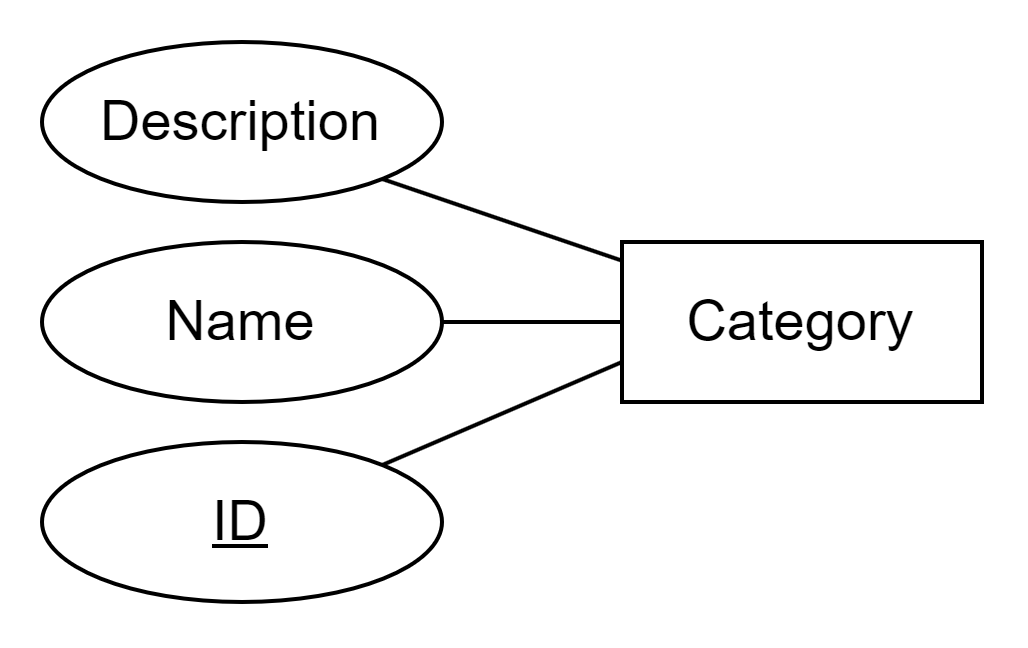
\includegraphics[scale = 0.20]{img/db/category.png}
    \vspace{1cm}
    \caption{Chi tiết thực thể \textbf{Category}}
    \label{fig:taskAssignment}
\end{figure}

\newpage
Các thuộc tính chính của thực thể \textbf{Category}
\begin{itemize}
    \item Description: Mô tả danh mục
    \item ID: ID định danh danh mục
    \item Name: Tên danh mục
\end{itemize}

\begin{figure}[h]
    \centering
    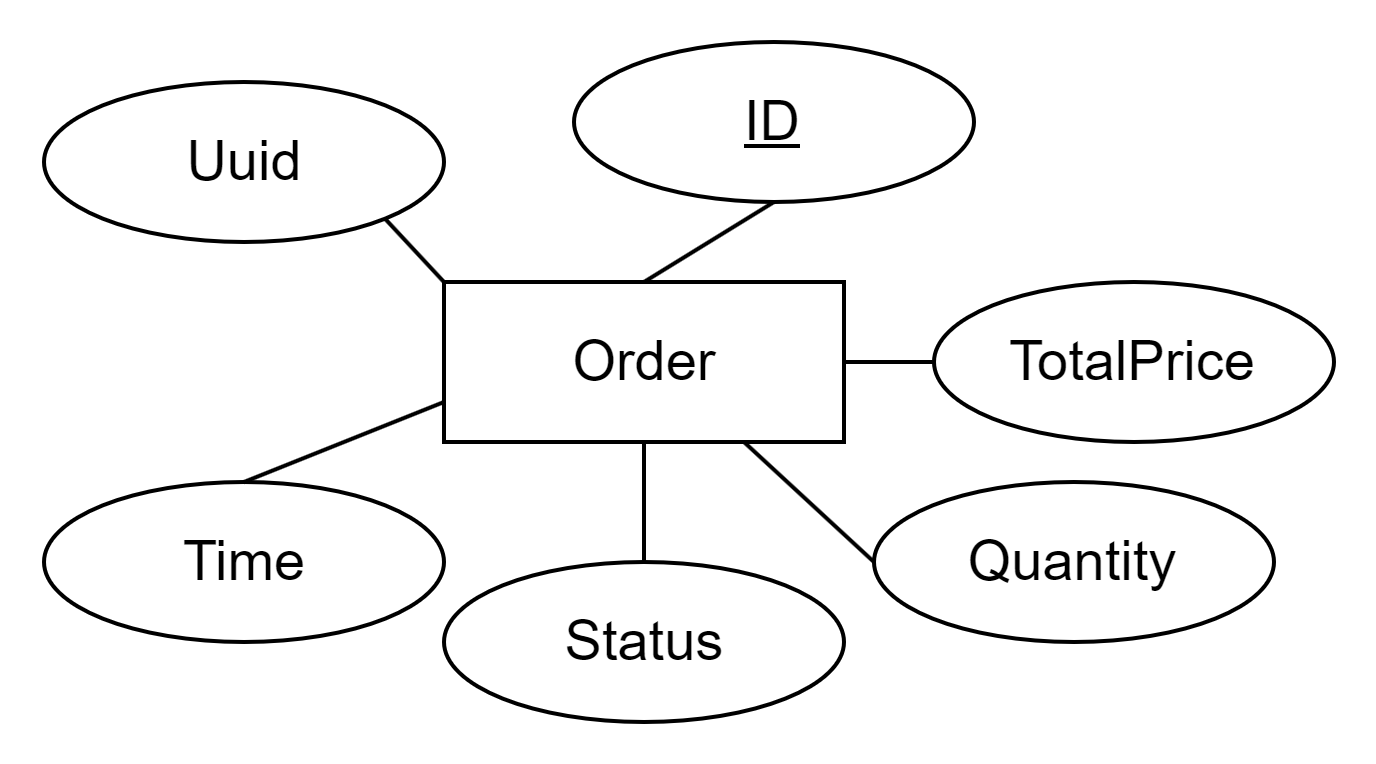
\includegraphics[scale = 0.20]{img/db/order.png}
    \vspace{1cm}
    \caption{Chi tiết thực thể \textbf{Order}}
    \label{fig:taskAssignment}
\end{figure}
Các thuộc tính chính của thực thể \textbf{Order}
\begin{itemize}
    \item Time: Ngày đặt hàng
    \item ID: ID định danh thực thể
    \item Uuid: Mã đơn hàng
    \item Status: Trạng thái đơn hàng
    \item Quantity: số lượng hàng
    \item TotalPrice: Tổng giá trị đơn hàng
\end{itemize}

\newpage
\begin{figure}[h]
    \centering
    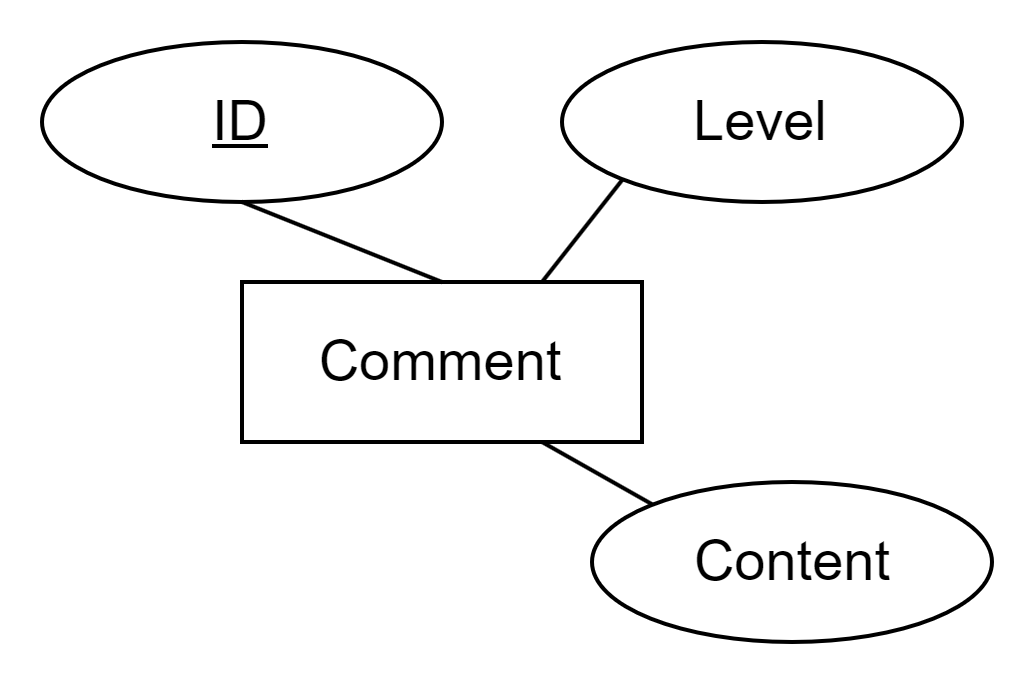
\includegraphics[scale = 0.20]{img/db/comment.png}
    \vspace{1cm}
    \caption{Chi tiết thực thể \textbf{Comment}}
    \label{fig:taskAssignment}
\end{figure}
Các thuộc tính chính của thực thể \textbf{Comment}
\begin{itemize}
    \item Level: Cấp độ của mình luận, mặc định "1". 1 bình luận có thể gọi đệ quy nhau, dẫn tới cấp độ tăng lên. 
    \item ID: ID định danh bình luận
    \item Content: Nội dung của bình luận.
\end{itemize}

\begin{figure}[h]
    \centering
    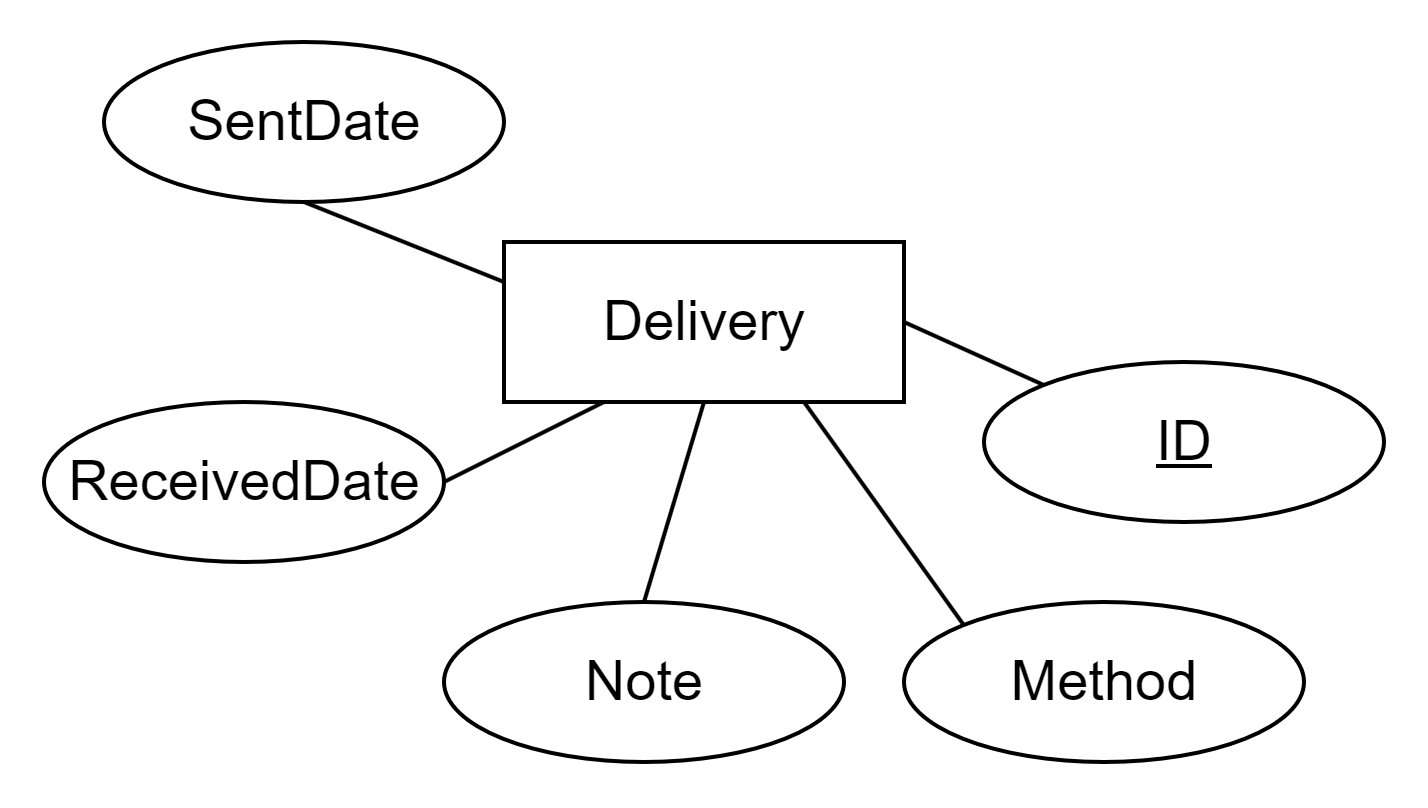
\includegraphics[scale = 0.20]{img/db/delivery.png}
    \vspace{1cm}
    \caption{Chi tiết thực thể \textbf{Delivery}}
    \label{fig:taskAssignment}
\end{figure}

Các thuộc tính chính của thực thể \textbf{Delivery}
\begin{itemize}
    \item SentDate: Ngày gửi hàng
    \item ID: ID định danh thực thể
    \item ReceivedDate: Ngày nhận hàng
    \item Note: Ghi chú khi gửi hàng
    \item Method: Phương thức gửi hàng
\end{itemize}

\newpage
\begin{figure}[h]
    \centering
    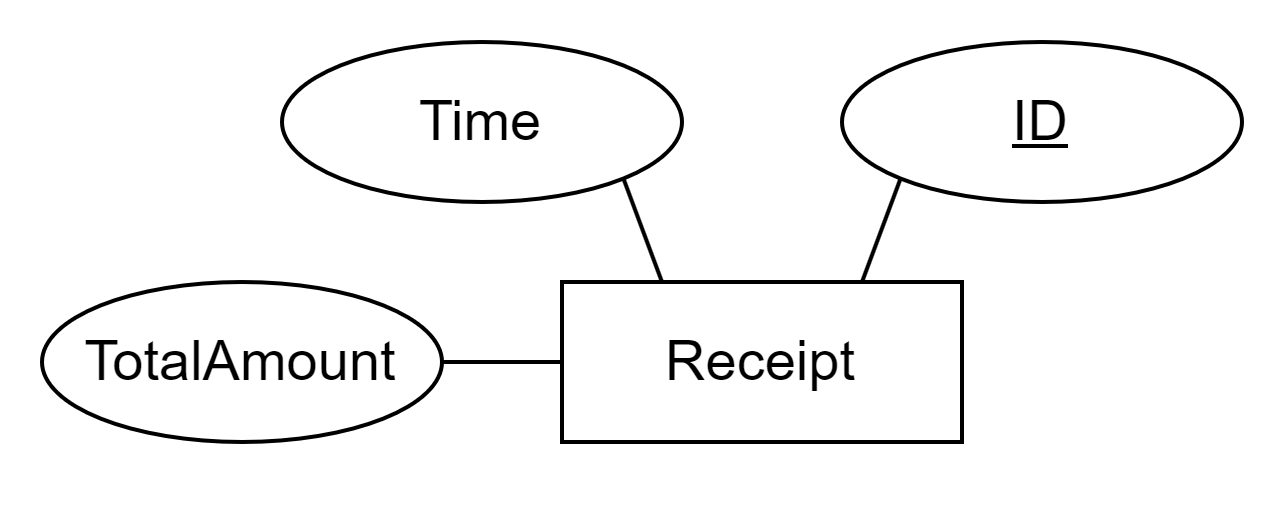
\includegraphics[scale = 0.20]{img/db/receipt.png}
    \vspace{1cm}
    \caption{Chi tiết thực thể \textbf{Receipt}}
    \label{fig:taskAssignment}
\end{figure}
Các thuộc tính chính của thực thể \textbf{Receipt}
\begin{itemize}
    \item Time: Thời gian xuất hóa đơn
    \item ID: ID định danh thực thể
    \item TotalAmount: Tổng giá trị hóa đơn
\end{itemize}

\begin{figure}[h]
    \centering
    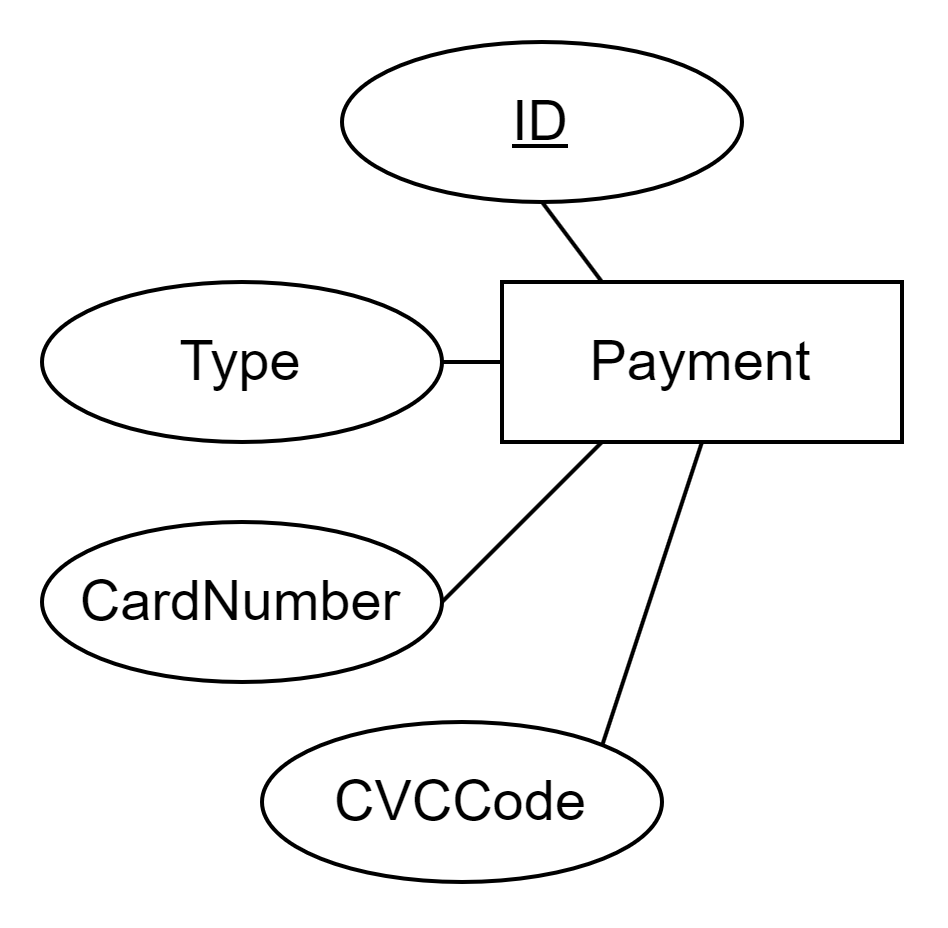
\includegraphics[scale = 0.20]{img/db/payment.png}
    \vspace{1cm}
    \caption{Chi tiết thực thể \textbf{Payment}}
    \label{fig:taskAssignment}
\end{figure}

Các thuộc tính chính của thực thể \textbf{Payment}
\begin{itemize}
    \item Type: Loại Phương thức thanh toán, (Visa, Mastercard ...)
    \item ID: ID định danh thực thể
    \item CardNumber: Số thẻ thanh toán
    \item CVCCode: Chữ kí thẻ thanh toán
\end{itemize}

\newpage
\begin{figure}[h]
    \centering
    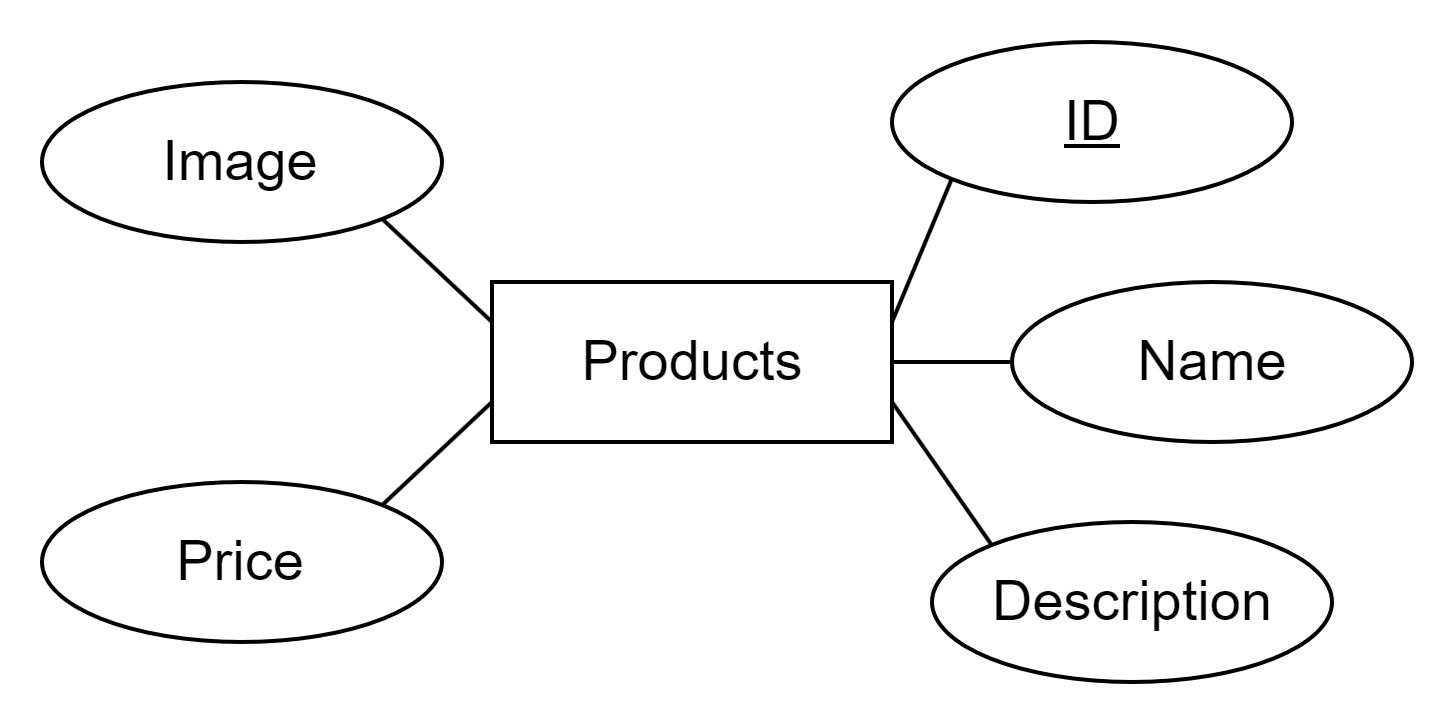
\includegraphics[scale = 0.20]{img/db/products.png}
    \vspace{1cm}
    \caption{Chi tiết thực thể \textbf{Products}}
    \label{fig:taskAssignment}
\end{figure}
Các thuộc tính chính của thực thể \textbf{Products}
\begin{itemize}
    \item Image: URL Hình ảnh của sản phẩm
    \item ID: ID định danh sản phẩm
    \item Price: Giá của sản phẩm
    \item Name: Tên của sản phẩm
    \item Description: Mô tả sản phẩm
\end{itemize}


\begin{figure}[h]
    \centering
    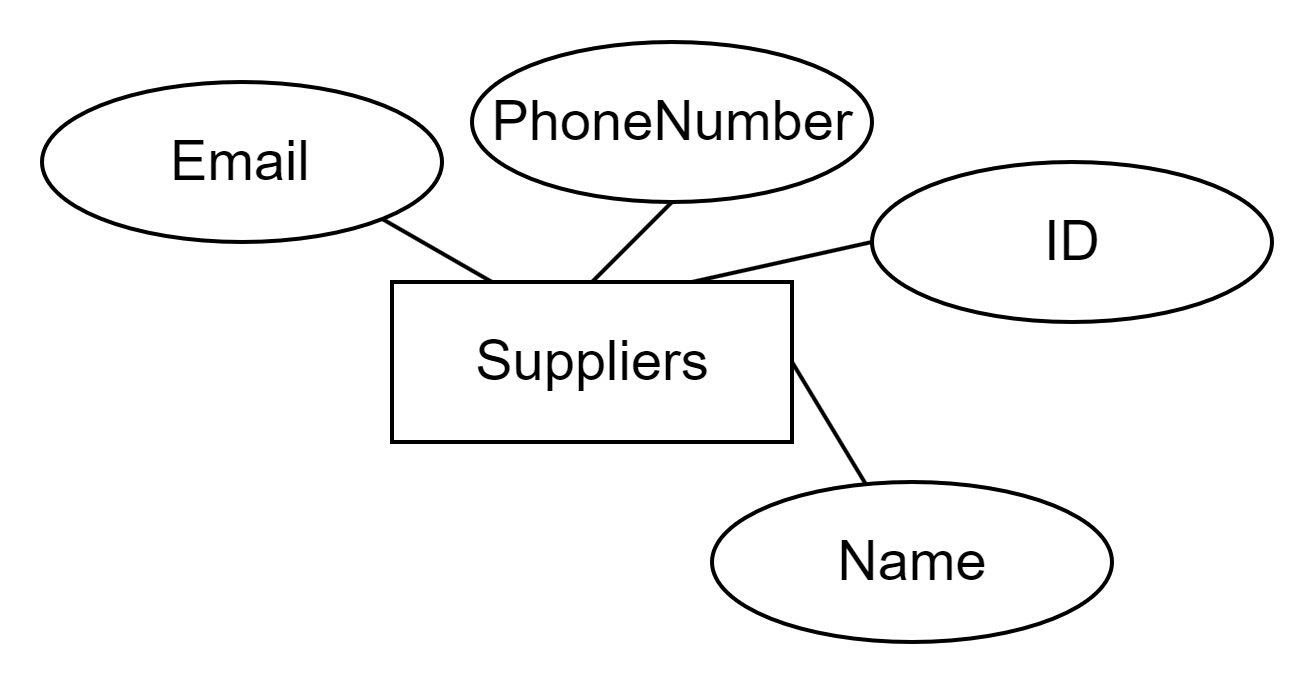
\includegraphics[scale = 0.20]{img/db/suppliers.png}
    \vspace{1cm}
    \caption{Chi tiết thực thể \textbf{Suppliers}}
    \label{fig:taskAssignment}
\end{figure}
Các thuộc tính chính của thực thể \textbf{Suppliers}
\begin{itemize}
    \item Name: Tên nhà cung cấp
    \item ID: ID định danh thực thể
    \item PhoneNumber: Số điện thoại của nhà cung cấp
    \item Email: Email của nhà cung cấp
\end{itemize}

\newpage
\subsection{Thiết kế cơ sở dữ liệu vật lý}
\newpage
\section{Class Diagram}
\subsection{Class Diagram cho service Customer}
\begin{figure}[h]
    \centering
    \rotatebox[origin=c]{-90}{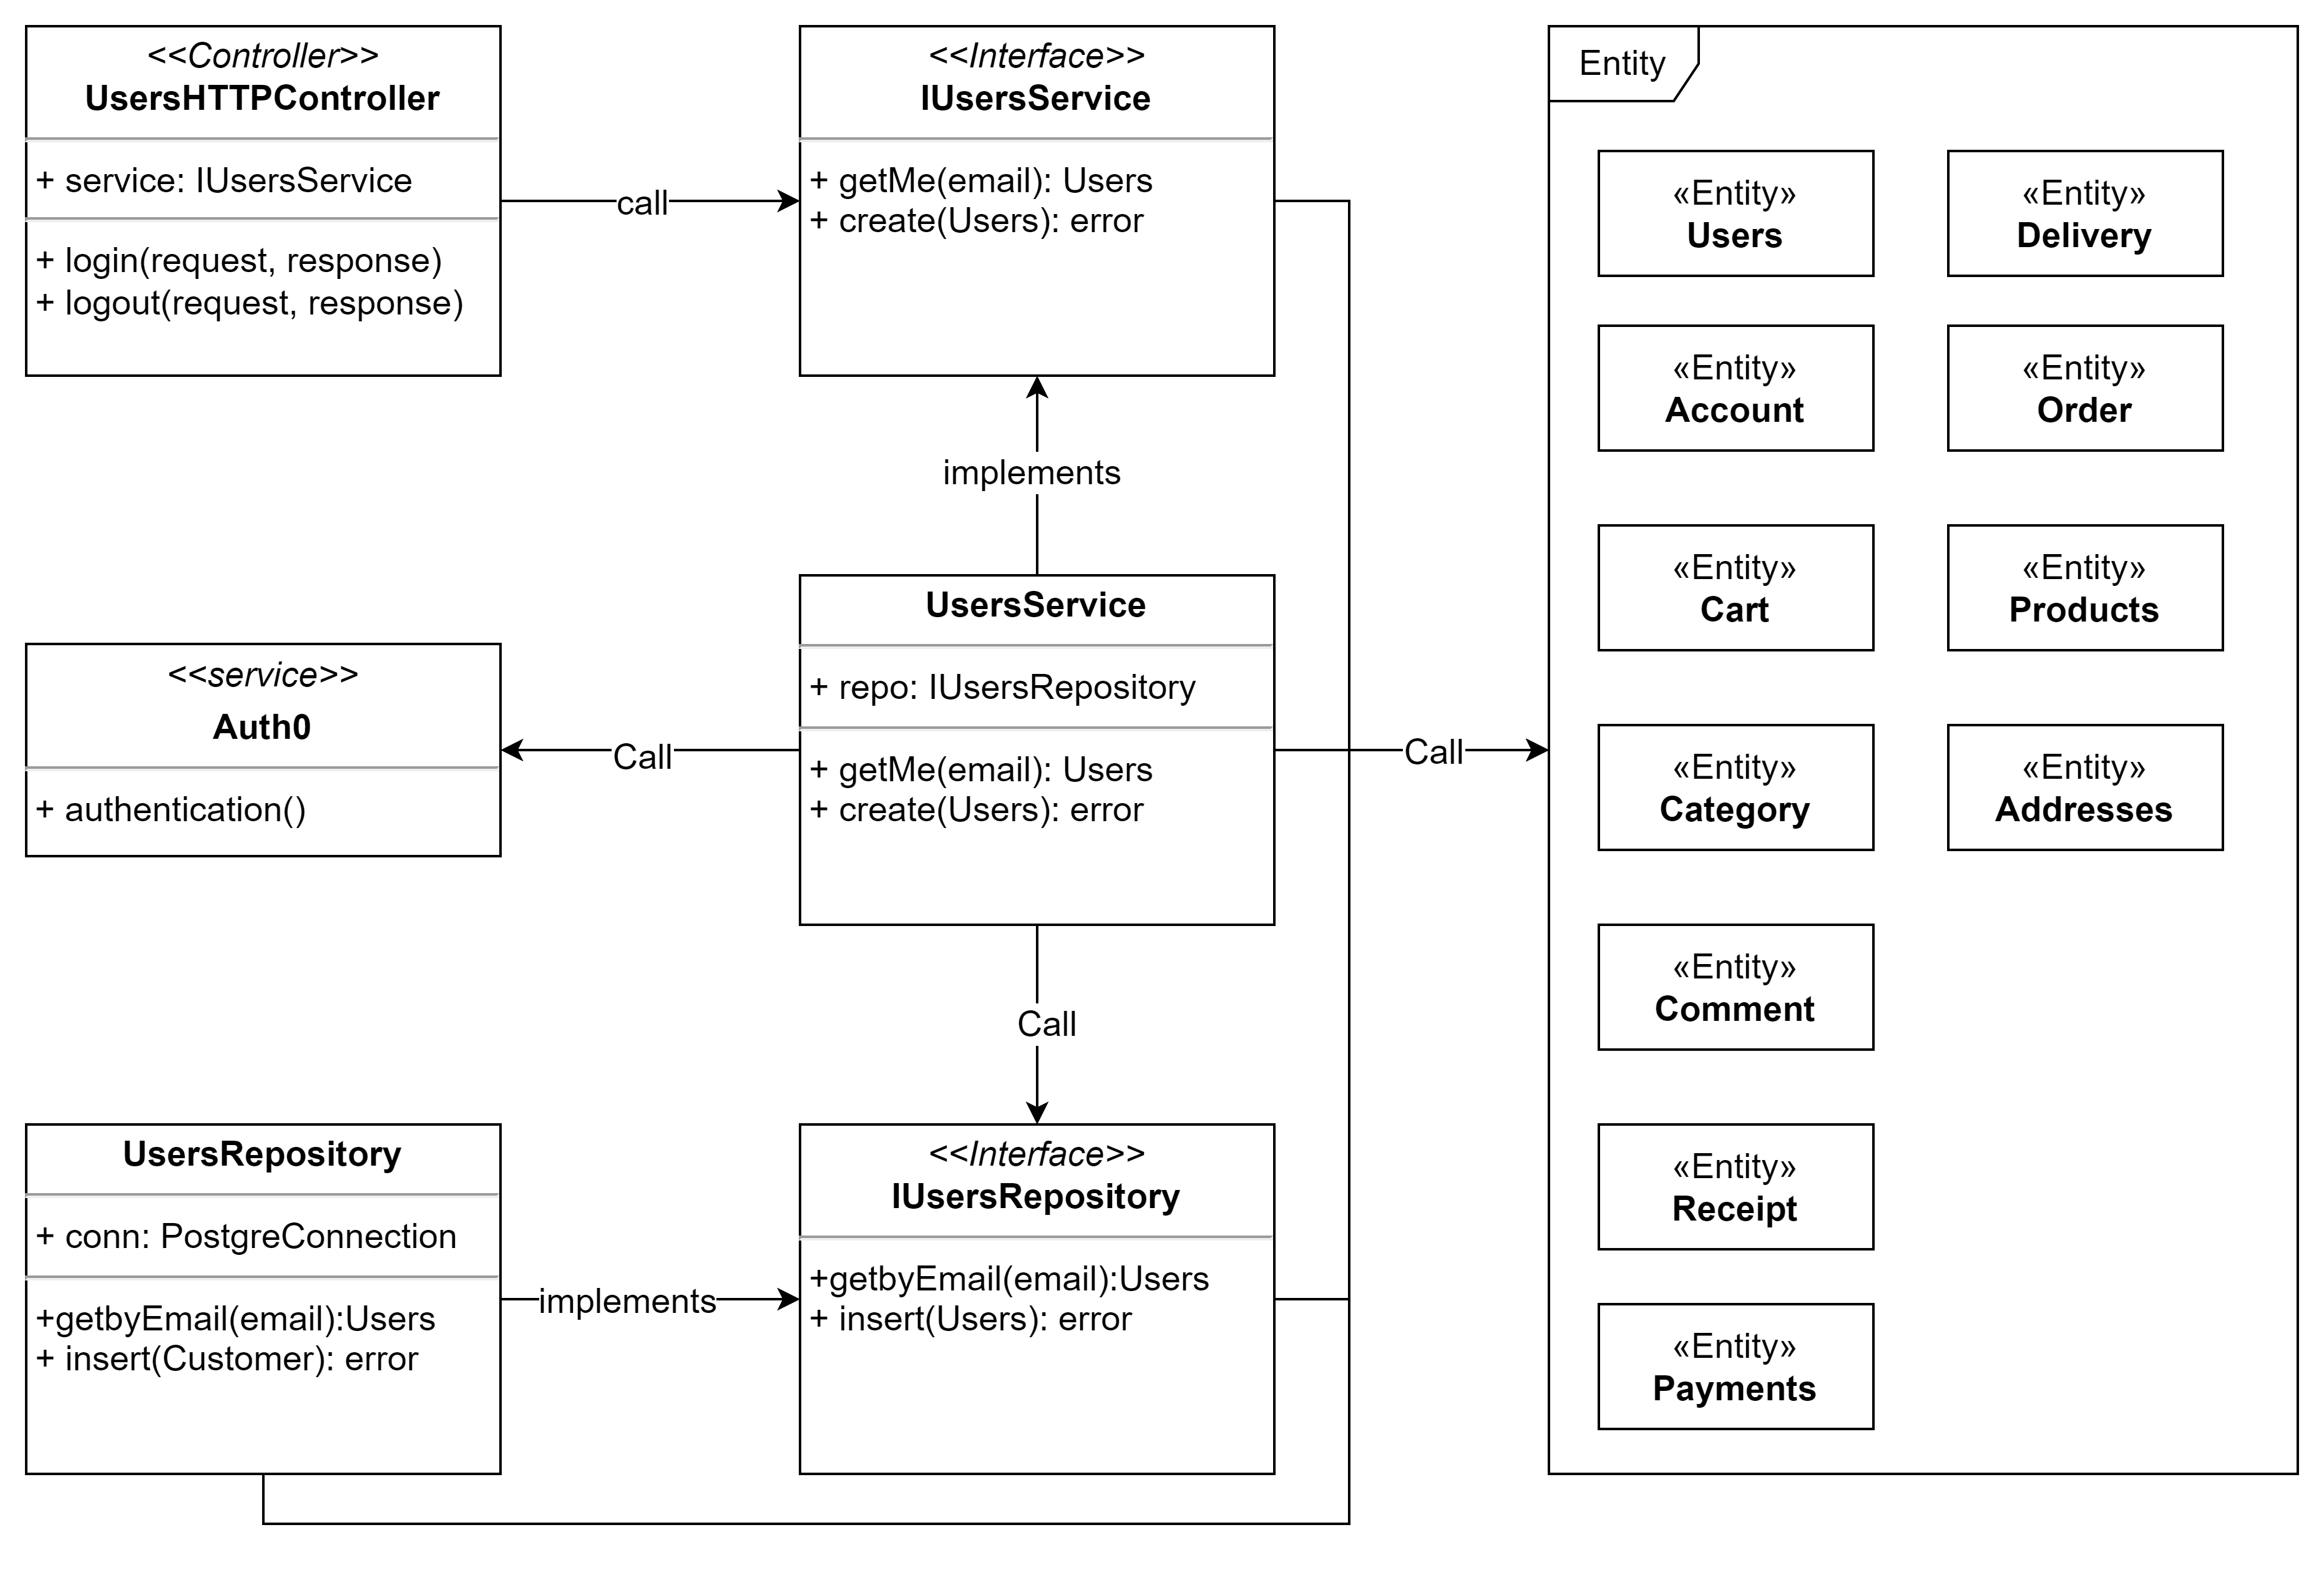
\includegraphics[width=18cm]{img/class/users.png}}
    \vspace{0.6cm}
    \caption{Class Diagram cho kiến trúc hệ thống}
    \label{fig:taskAssignment}
\end{figure}

\newpage
\section{Triển khai hệ thống}
\begin{figure}[h]
    \centering
    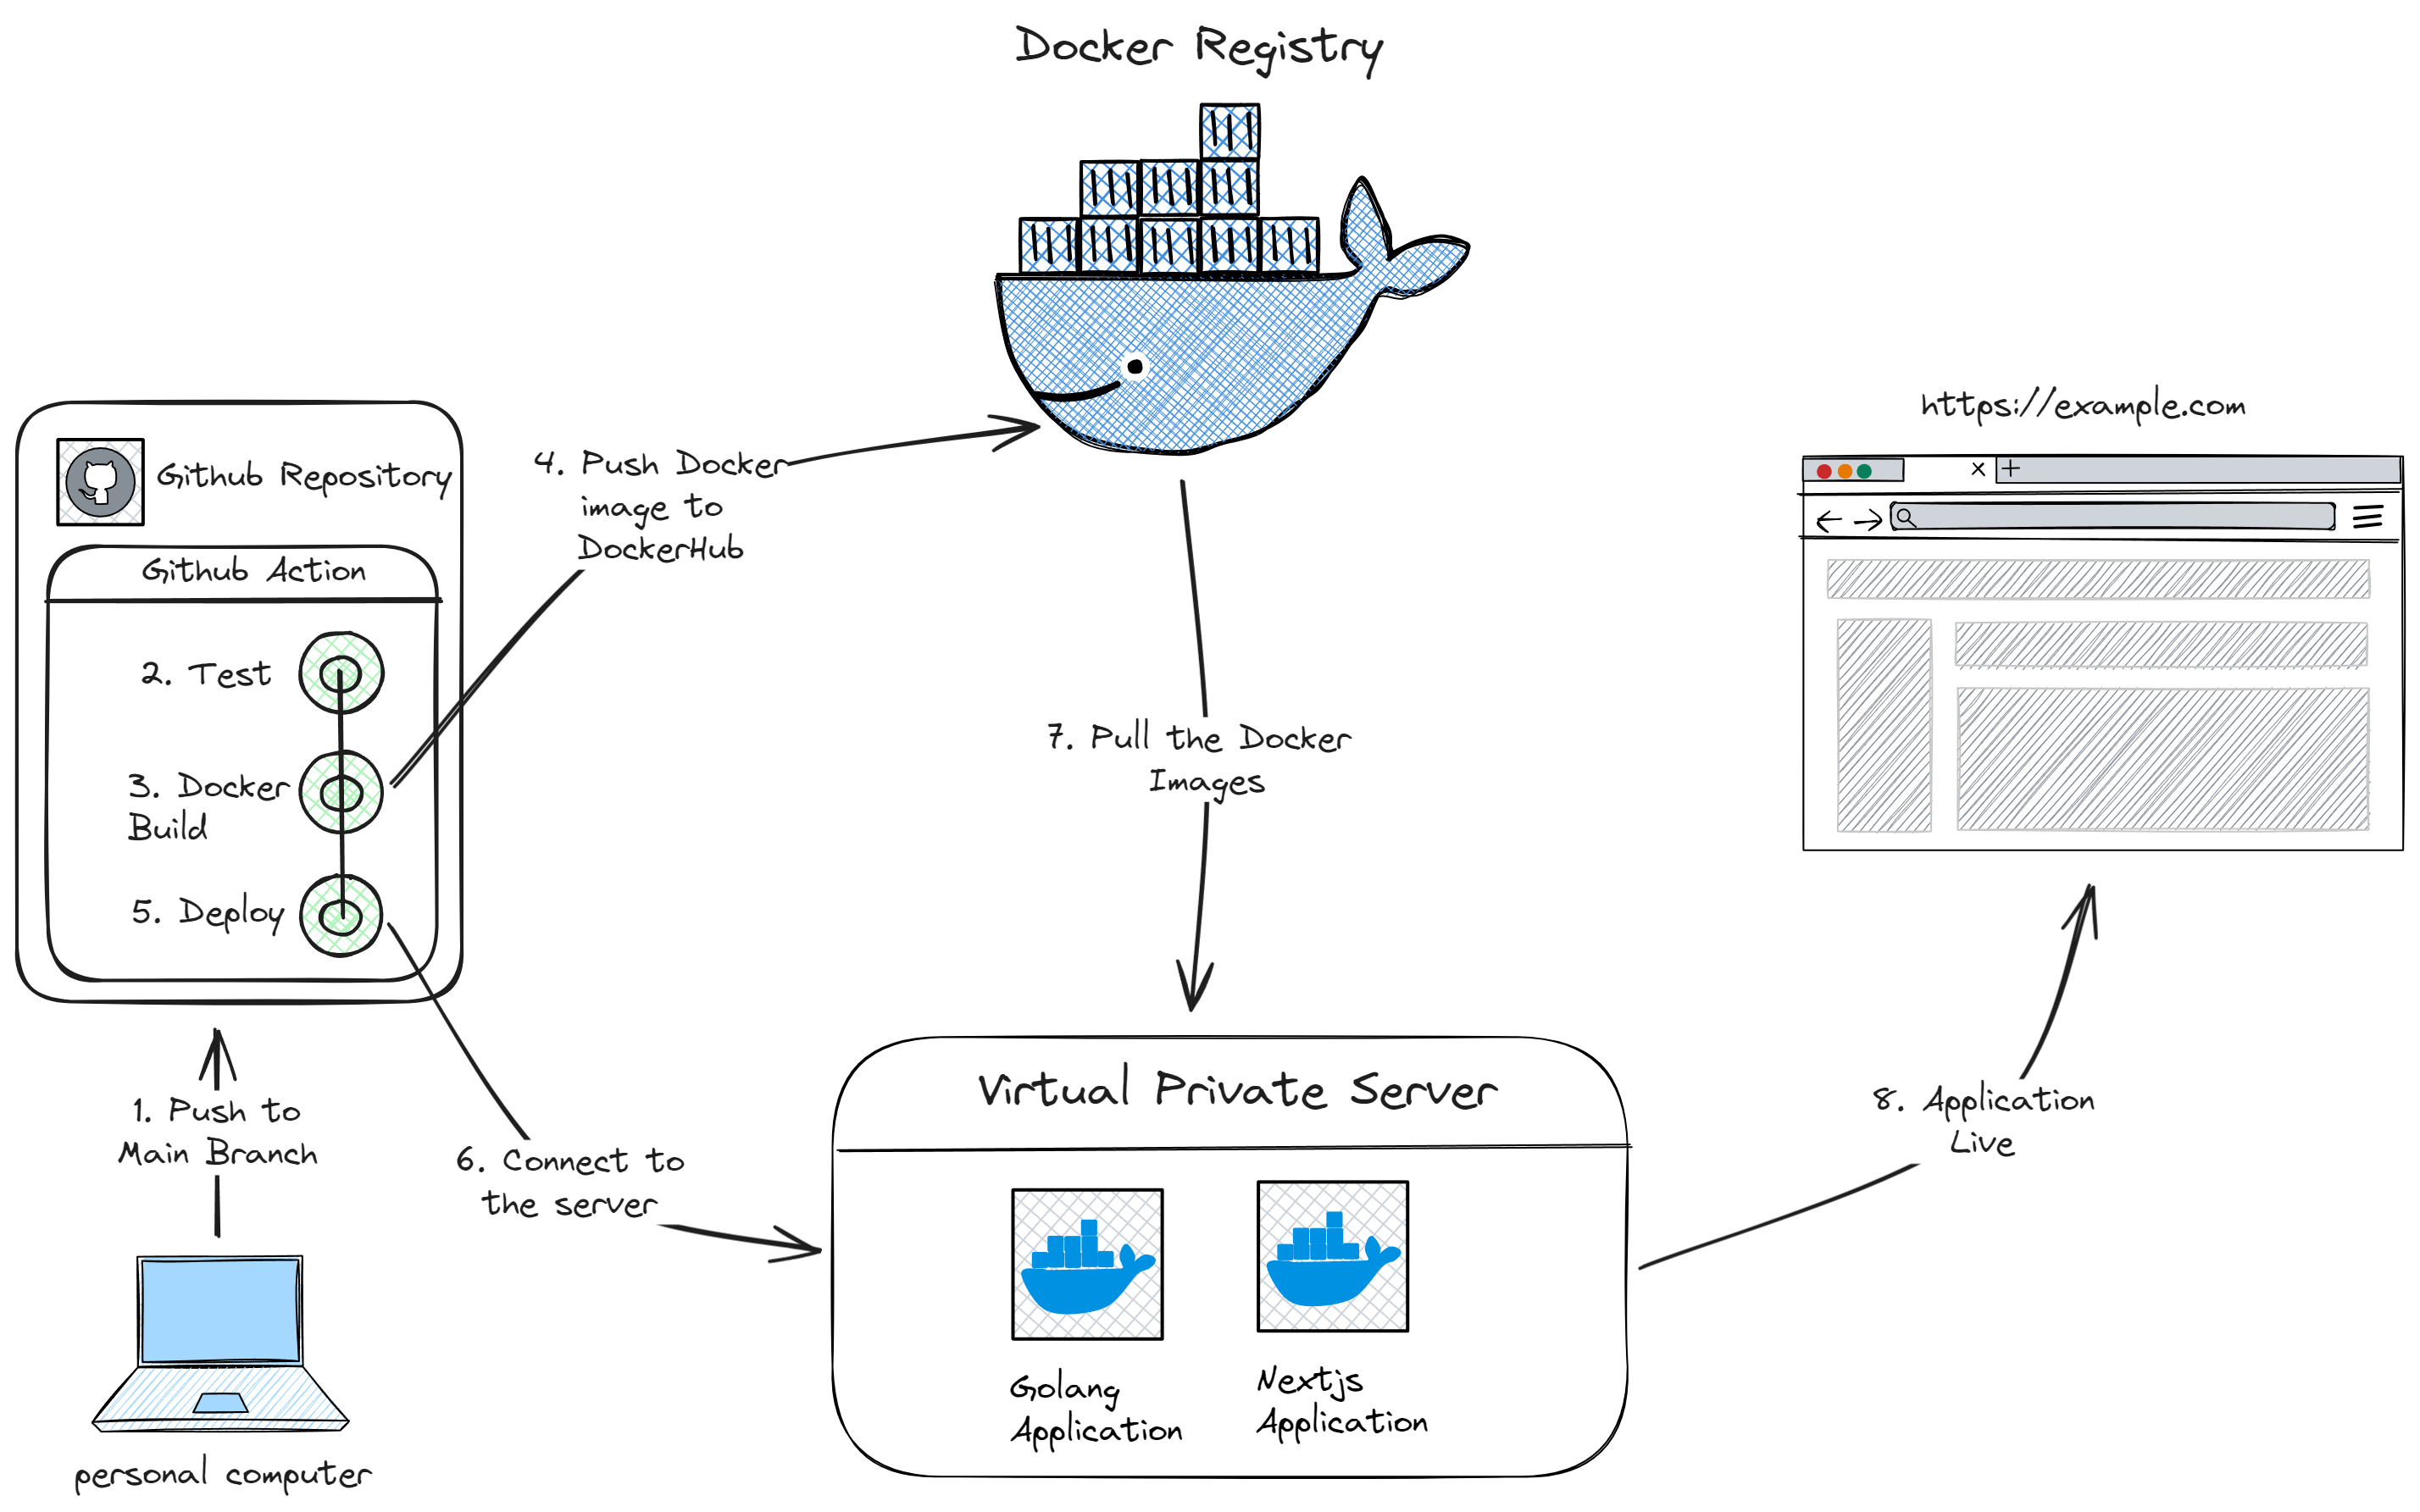
\includegraphics[scale = 0.17]{img/workflow.png}
    \vspace{1cm}
    \caption{Tổng quan luồn triển khai hệ thống}
    \label{fig:taskAssignment}
\end{figure}
\section{Giao diện và trải nghiệm người dùng}